 \section{Part C}
 \begin{itemize}
 \item
Now quantify the agreement of the clusters with the party affiliations (for example, using the mutual information between cluster membership and party affiliation). 
\item
Repeat the clustering analysis using the first two principal components (instead of all 16 votes). Again, quantify the agreement of the clusters with the party affiliations. Which clustering (using principal components vs. using all 16 votes) agrees with the party affiliations more? Comment on why this might be the case. 
\end{itemize}

-----\\

To quantify the agreement of the clusters with the party affiliations, I used mutual information as the example suggests. The visualization code is shown below for the comparison visual of the different clusterings:

\begin{verbatim}
def plot_comparison(votes_pca: np.ndarray, cluster_labels_full: np.ndarray,
                   cluster_labels_pca: np.ndarray, output_filename: str):
    """
    Plots side-by-side comparison of clustering on full data vs PCs.
    
    :param votes_pca: pca-transformed data
    :type votes_pca: np.ndarray
    :param cluster_labels_full: Cluster assignments from full data
    :type cluster_labels_full: np.ndarray
    :param cluster_labels_pca: Cluster assignments from pca data
    :type cluster_labels_pca: np.ndarray
    :param party_labels: Party affiliation labels
    :type party_labels: np.ndarray
    :param output_filename: Filename for output figure
    :type output_filename: str
    """
    sns.set_style("whitegrid")
    sns.set_palette("muted")
    _, (ax1, ax2) = plt.subplots(1, 2, figsize=(16, 6))
    
    cluster_colors = ['purple', 'gold']
    
    cluster_0_full_mean_pc1 = np.mean(votes_pca[cluster_labels_full == 0, 0])
    cluster_1_full_mean_pc1 = np.mean(votes_pca[cluster_labels_full == 1, 0])
    flip_full = cluster_0_full_mean_pc1 > cluster_1_full_mean_pc1
    
    cluster_0_pca_mean_pc1 = np.mean(votes_pca[cluster_labels_pca == 0, 0])
    cluster_1_pca_mean_pc1 = np.mean(votes_pca[cluster_labels_pca == 1, 0])
    flip_pca = cluster_0_pca_mean_pc1 > cluster_1_pca_mean_pc1
    
    # Clusters on full data
    for cluster in range(2):
        mask = cluster_labels_full == cluster
        color_idx = 1 - cluster if flip_full else cluster
        ax1.scatter(votes_pca[mask, 0], votes_pca[mask, 1],
                   c=cluster_colors[color_idx], label=f'Cluster {cluster}',
                   alpha=0.6, s=50, edgecolor='white', linewidth=0.5)
    
    ax1.set_xlabel('PC1', fontsize=14, labelpad=15)
    ax1.set_ylabel('PC2', fontsize=14, labelpad=15)
    ax1.set_title('K-means on Full Data', fontsize=16, pad=20)
    ax1.legend(fontsize=10, loc='best')
    ax1.grid(True, alpha=0.3)
    
    # Clusters on pc1-pc2
    for cluster in range(2):
        mask = cluster_labels_pca == cluster
        color_idx = 1 - cluster if flip_pca else cluster
        ax2.scatter(votes_pca[mask, 0], votes_pca[mask, 1],
                   c=cluster_colors[color_idx], label=f'Cluster {cluster}',
                   alpha=0.6, s=50, edgecolor='white', linewidth=0.5)
    
    ax2.set_xlabel('PC1', fontsize=14, labelpad=15)
    ax2.set_ylabel('PC2', fontsize=14, labelpad=15)
    ax2.set_title('K-means on PC1-PC2', fontsize=16, pad=20)
    ax2.legend(fontsize=10, loc='best')
    ax2.grid(True, alpha=0.3)
    
    plt.tight_layout()
    os.makedirs("../figures", exist_ok=True)
    plt.savefig(f"../figures/{output_filename}", bbox_inches='tight', dpi=300)
\end{verbatim}

\begin{center}
\textbf{Figure 11:} Comparison visualization function for full data vs PCA clustering.
\end{center}

\begin{center}
  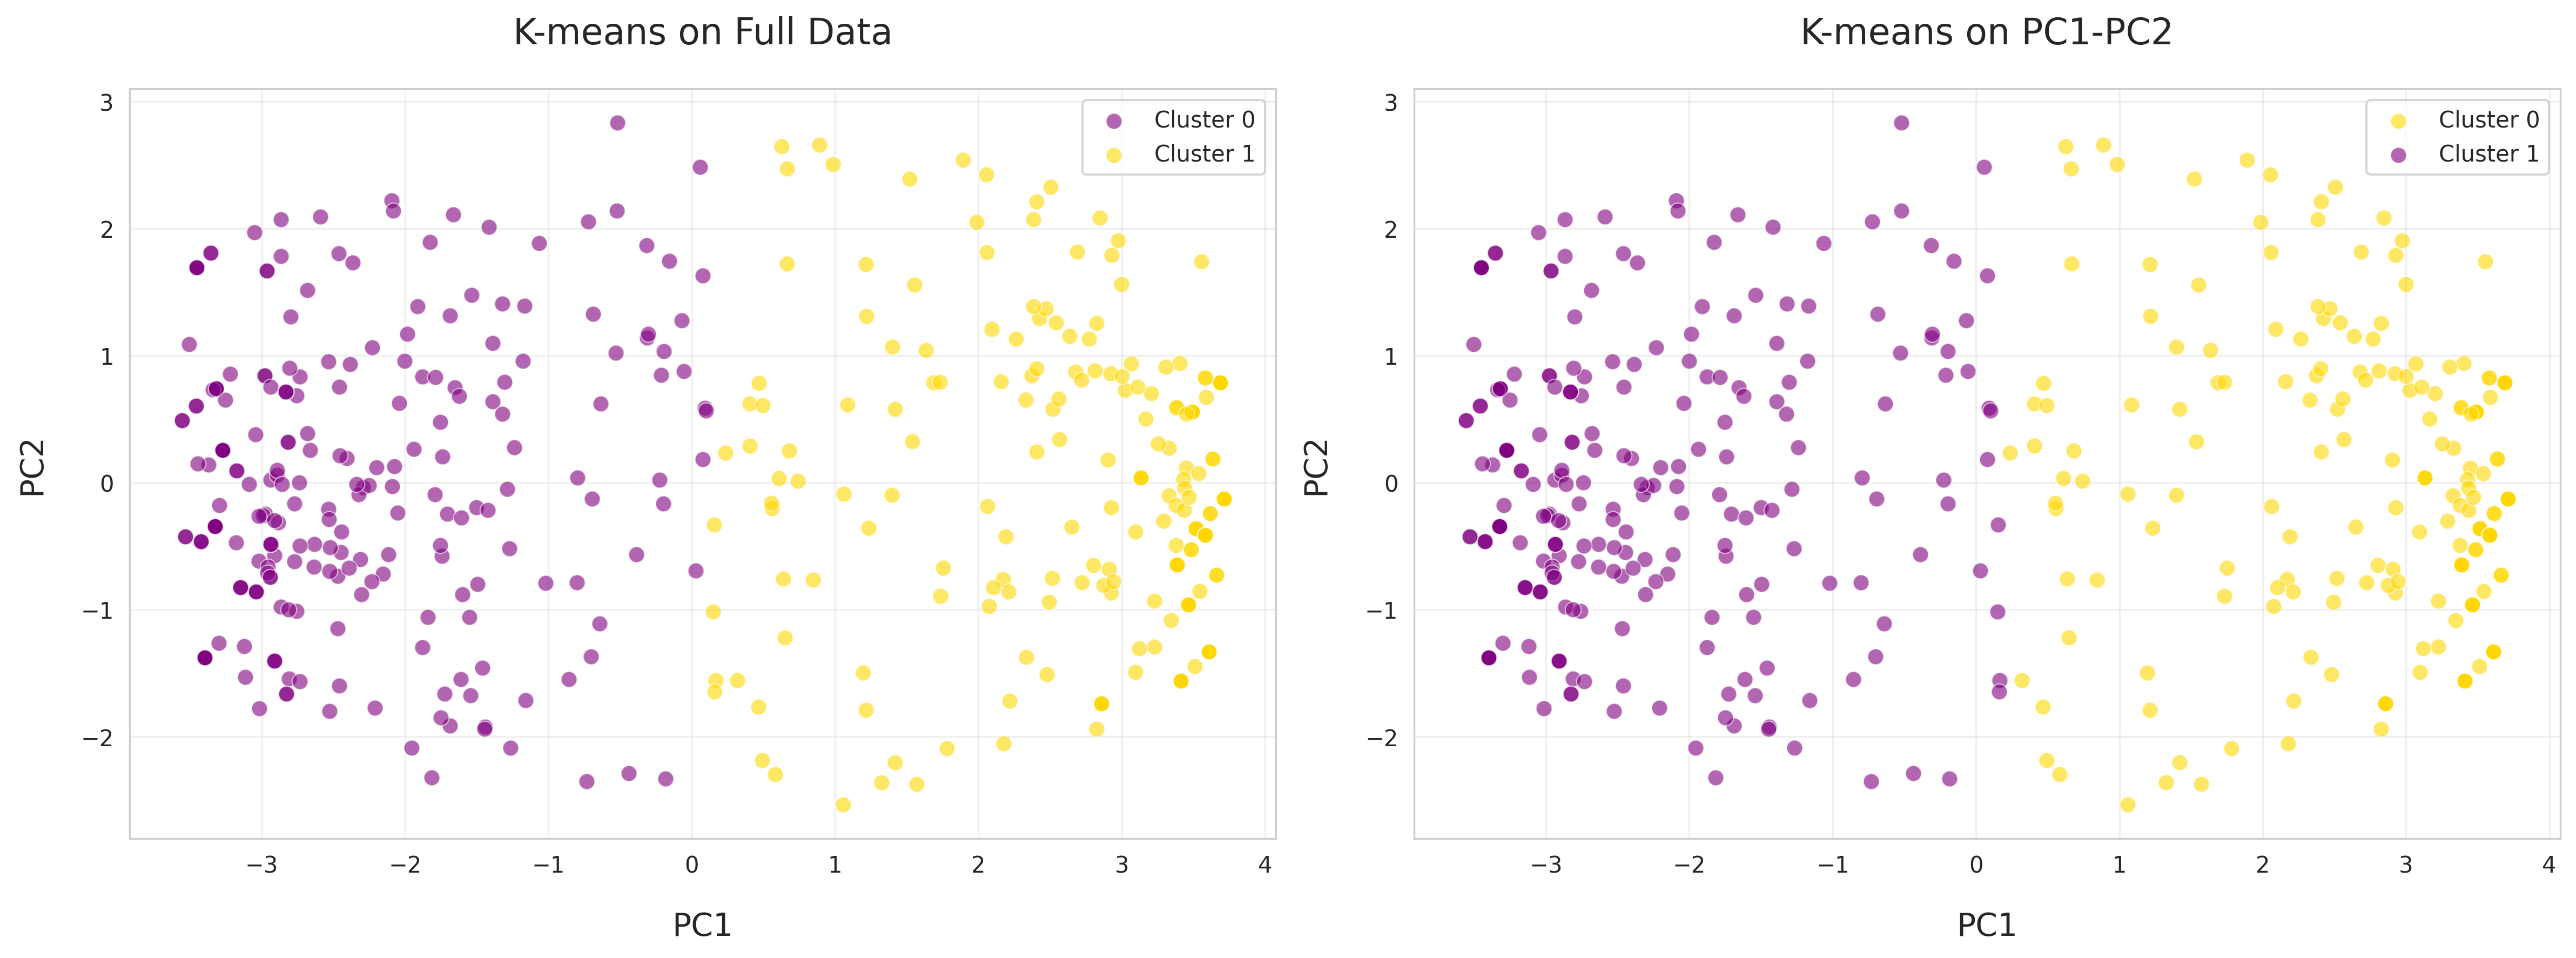
\includegraphics[width=0.95\textwidth]{figures/clustering_comparison.png}
  
  \textbf{Figure 13:} Side-by-side comparison of K-means clustering on 16 votes versus PC1-PC2 only.
\end{center}

The mutual information I obtained for the voting data and just the two PCs were 0.5097 and 0.4851 respectively. Both clusterings show decent agreement between the cluster assignments and the party affiliations, however the full data clustering shows just slightly better performance, as we would expect. I intended to show with the comparison visual the very slight differences in classification between the two approaches, which are readily apparent from the vertical party line down the PC1 origin boundary.\\

Regarding the result, PC1 and PC2 together explain 56.24\% of the variance in the voting data, whereas the rest of the information about voting patterns lies in all of the components that were left out. In excluding them, the clustering is based only on these two dominant directions of variance, so it makes sense that the clustering would be more inexact and less-representative of the subtler patterns of agreement and disagreement across all of the issues that may align certain individuals better with their actual party membership. It is nonetheless impressive though how similar of a clustering could be achieved just from the first two PCs, where on visual inspection, the two approaches only differed in classification of 4 members of Congress.

\newpage
